\documentclass[12pt,reqno]{amsart}
\usepackage{/Users/johnmyers/tex/handout,/Users/johnmyers/tex/customcommands,polynom}
\usepackage{caption}

\hdr{MAT 240}{28 Vector fields}

\begin{document}

\bigskip
\prob Sketch the following vector fields in $\bbr^2$.

\medskip
\begin{enumerate}
\item $\vec{F}(x,y) = \begin{bmatrix} 2 \\3\end{bmatrix}$ \vfill
\item $\vec{F}(x,y) = \begin{bmatrix}y \\0\end{bmatrix}$ \vfill
\item $\vec{F}(x,y) = \begin{bmatrix}x\\y\end{bmatrix}$ \vfill\newpage
\item $\vec{F}(x,y) = \begin{bmatrix} y \\ -x\end{bmatrix}$ \vfill
\item $\vec{F}(x,y) = \displaystyle\frac{x\vec{i} + y\vec{j}}{\sqrt{x^2+y^2}}$ \vfill
\end{enumerate}


\prob Match the vector fields in $\bbr^3$ to their formulas.

\bigskip
\begin{minipage}{0.3\textwidth}
\begin{enumerate}
\item $\vec{F}(x,y,z) = \begin{bmatrix}1\\2\\3\end{bmatrix}$\vspace{0.5in}
\item $\vec{F}(x,y,z) = \begin{bmatrix}1\\2\\z\end{bmatrix}$\vspace{0.5in}
\item $\vec{F}(x,y,z) = \begin{bmatrix}x\\y\\3\end{bmatrix}$\vspace{0.5in}
\item $\vec{F}(x,y,z) = \begin{bmatrix}x\\y\\z\end{bmatrix}$
\end{enumerate}
\end{minipage}
\begin{minipage}{0.7\textwidth}
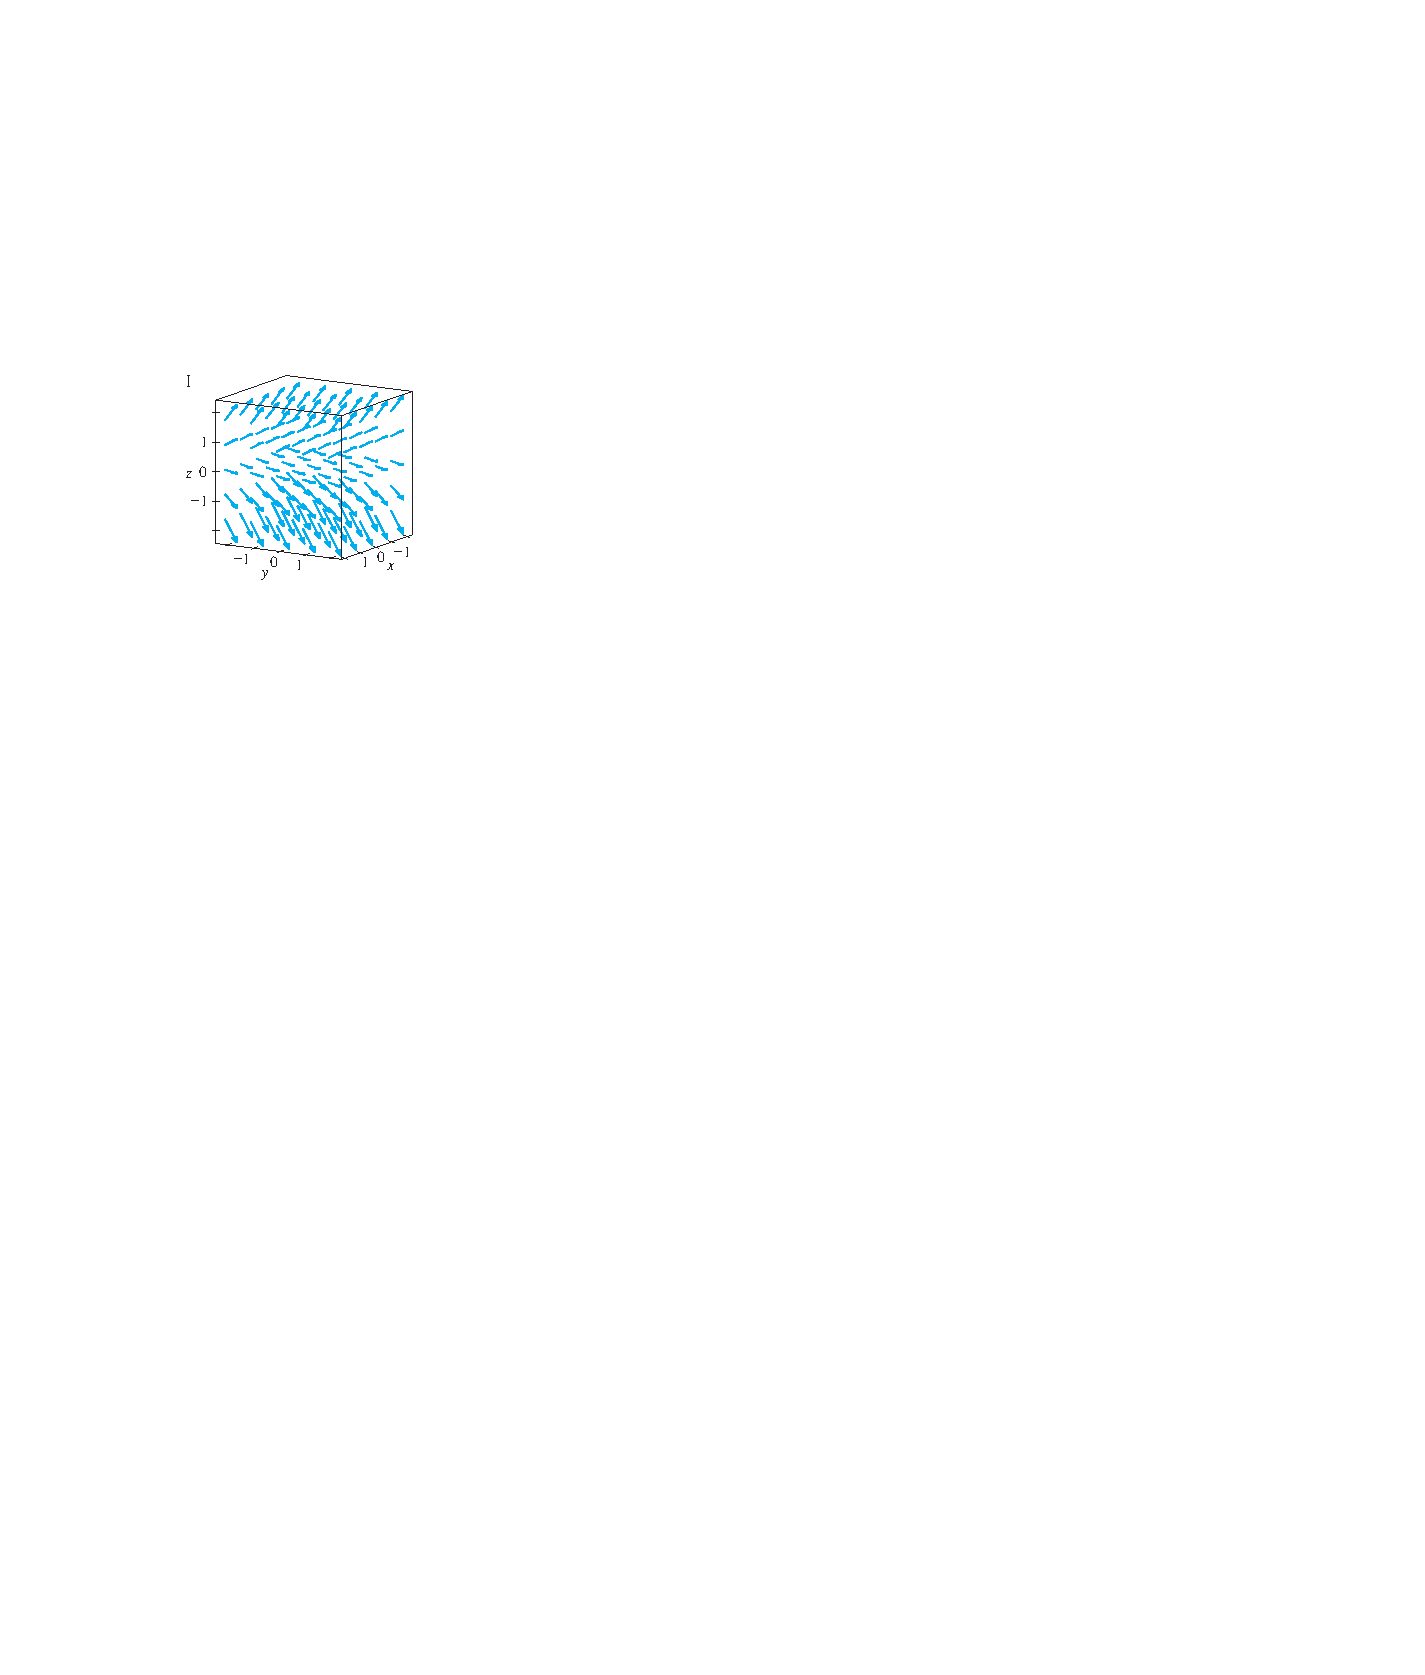
\includegraphics[scale=1.25]{I.pdf}
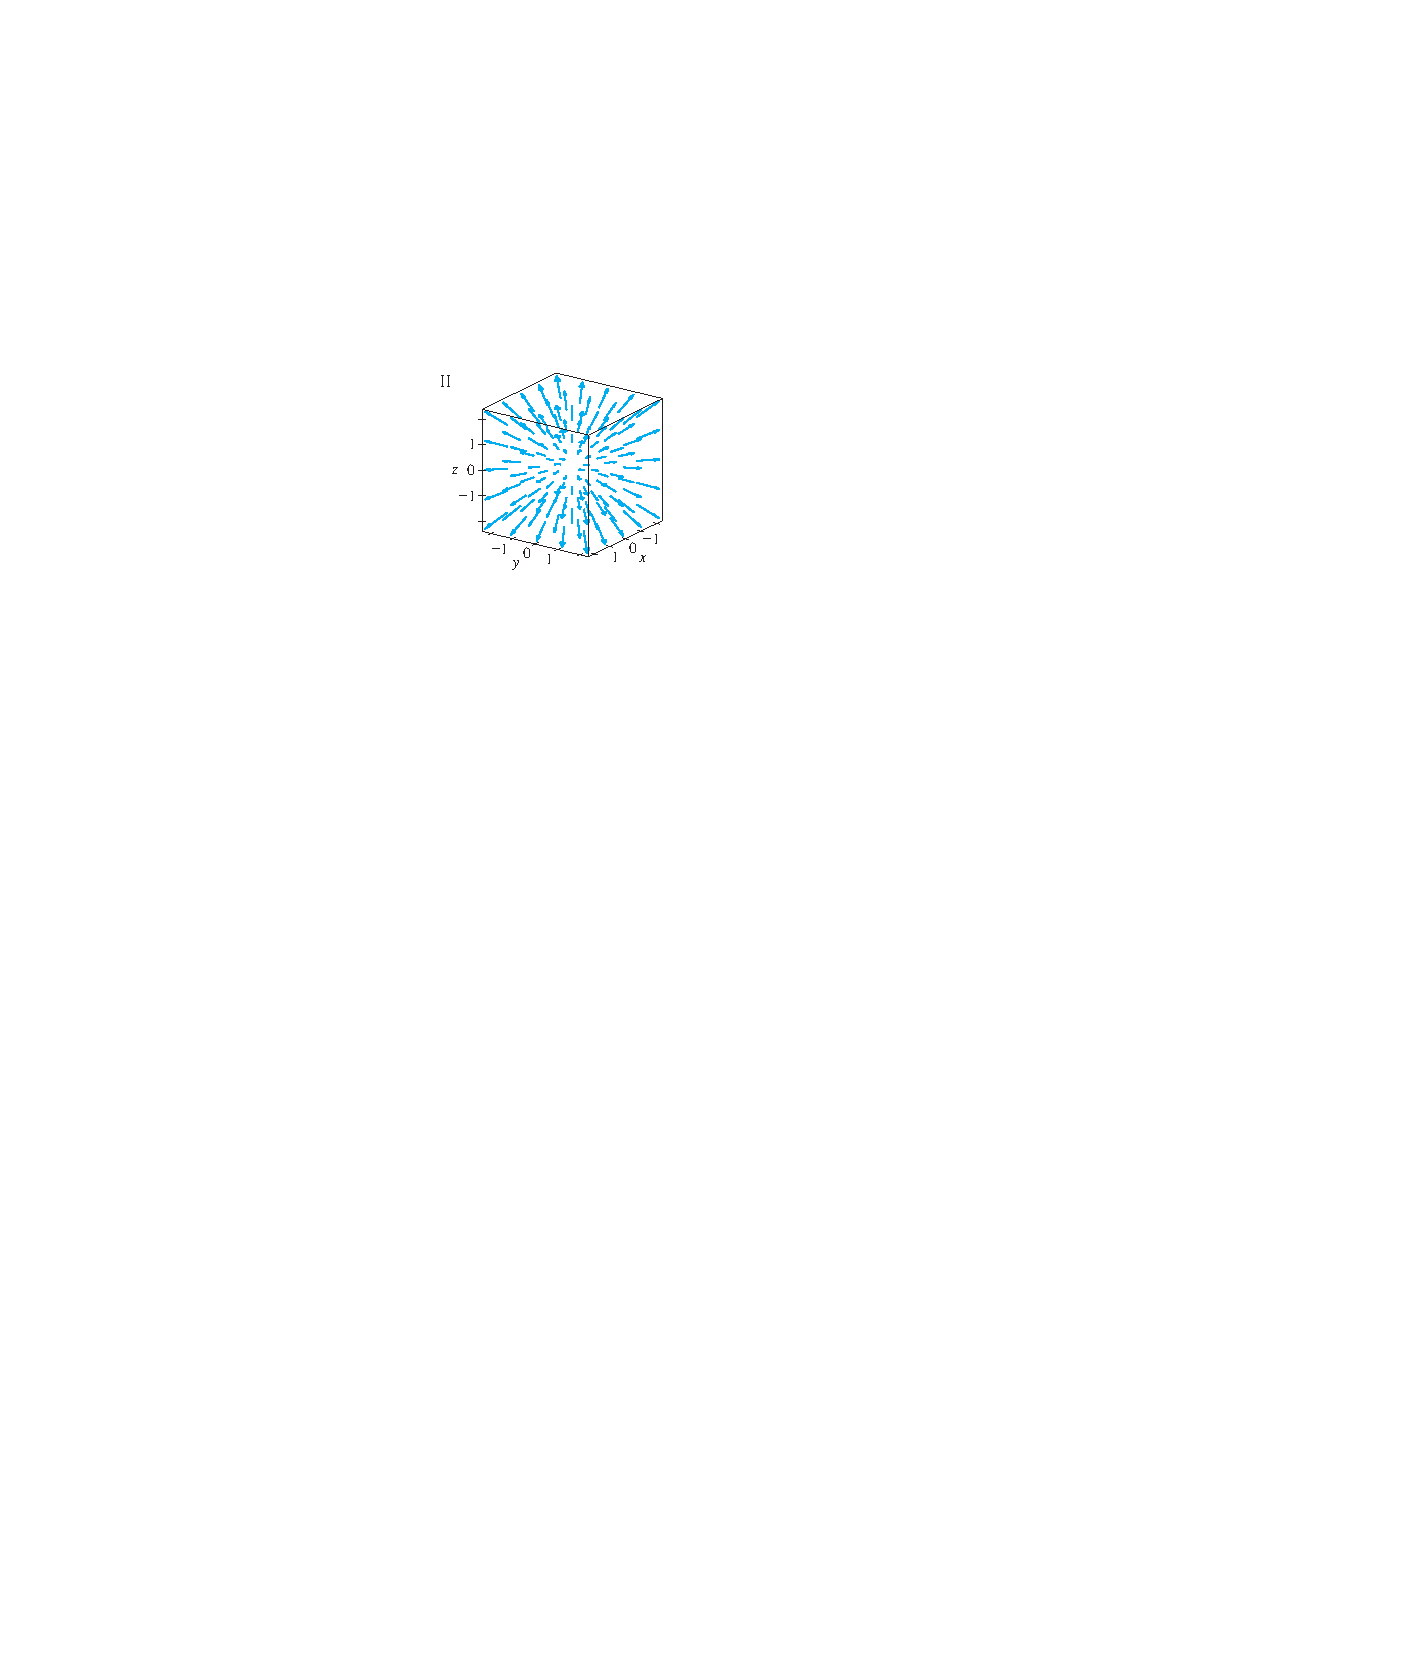
\includegraphics[scale=1.25]{II.pdf} \\
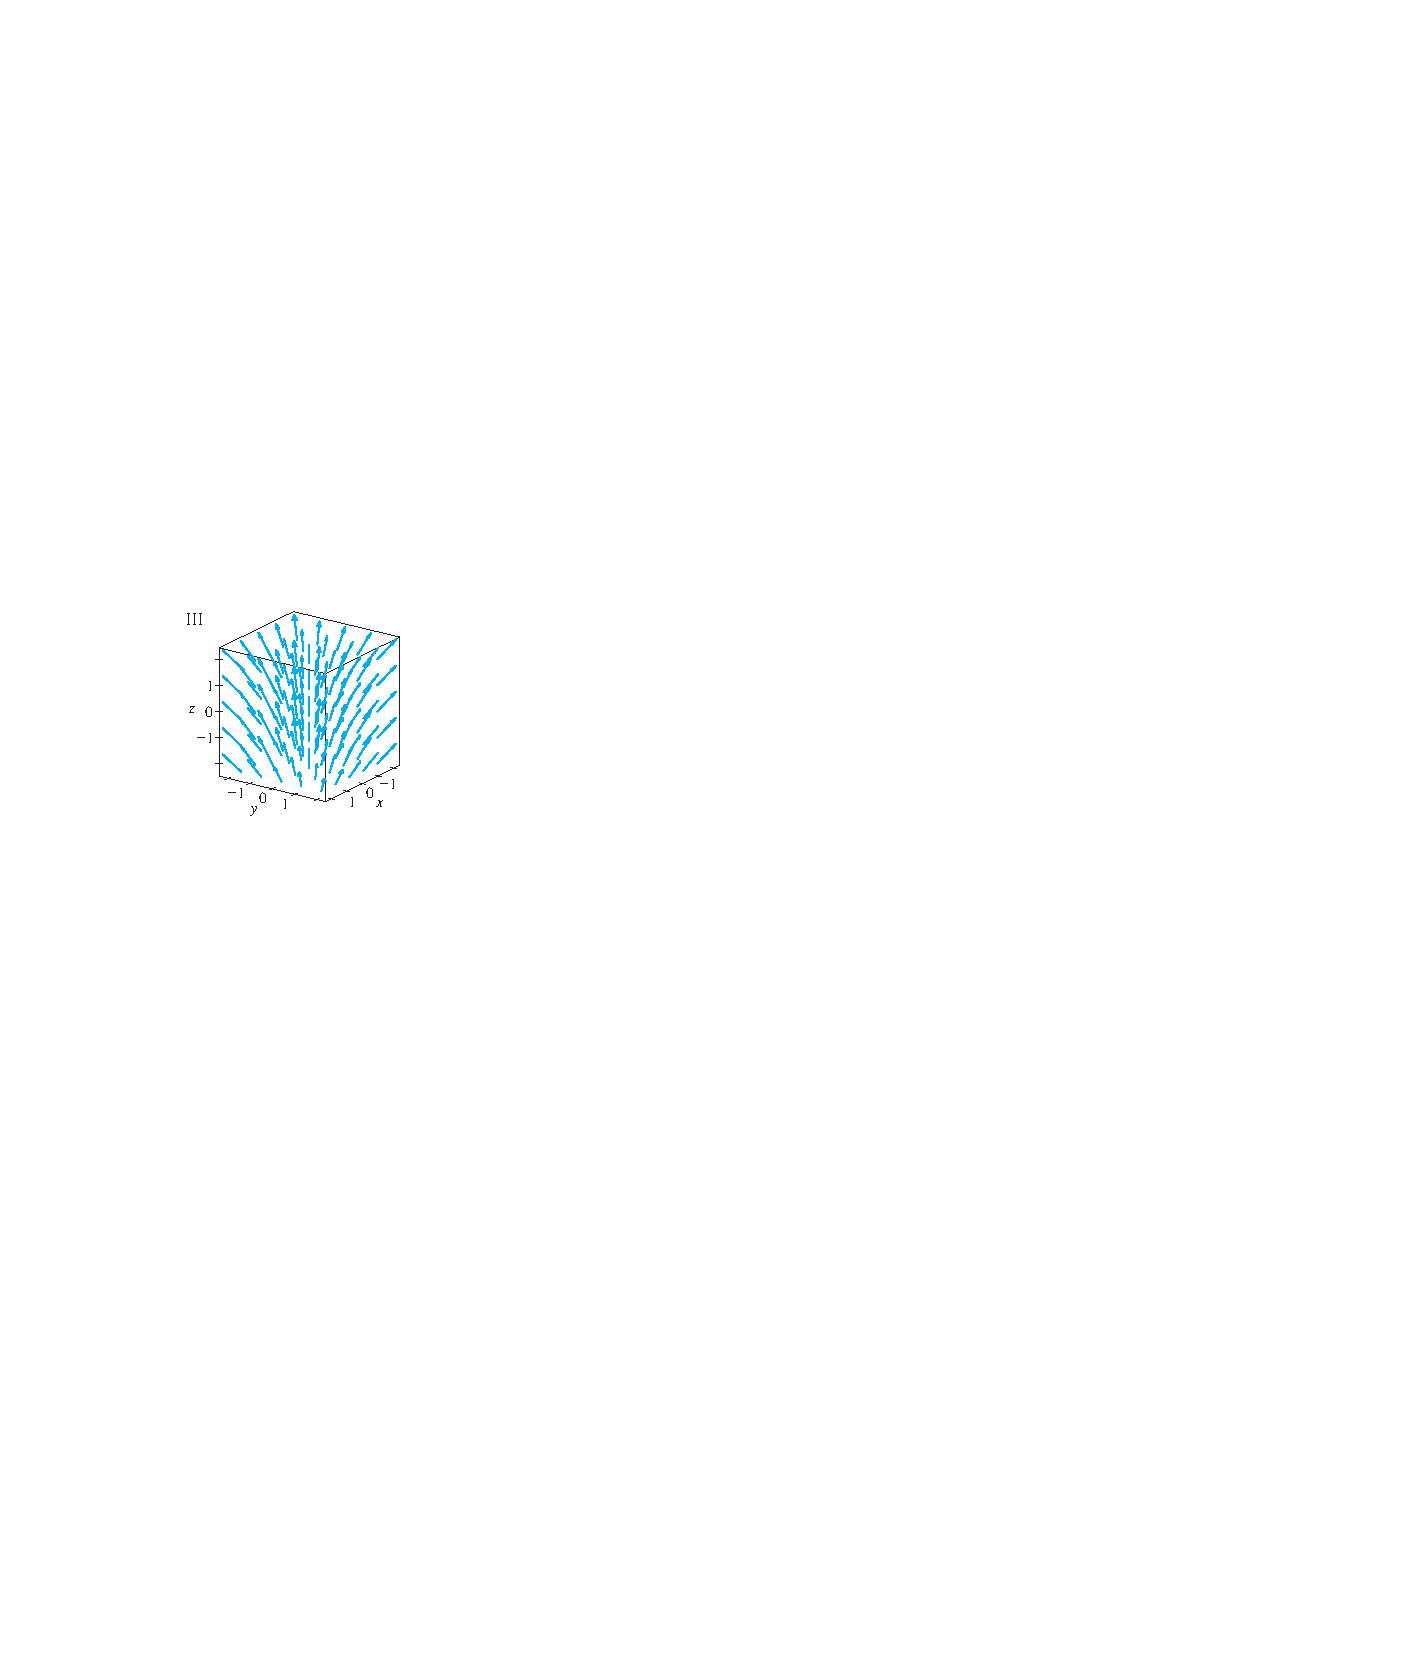
\includegraphics[scale=1.25]{III.pdf}
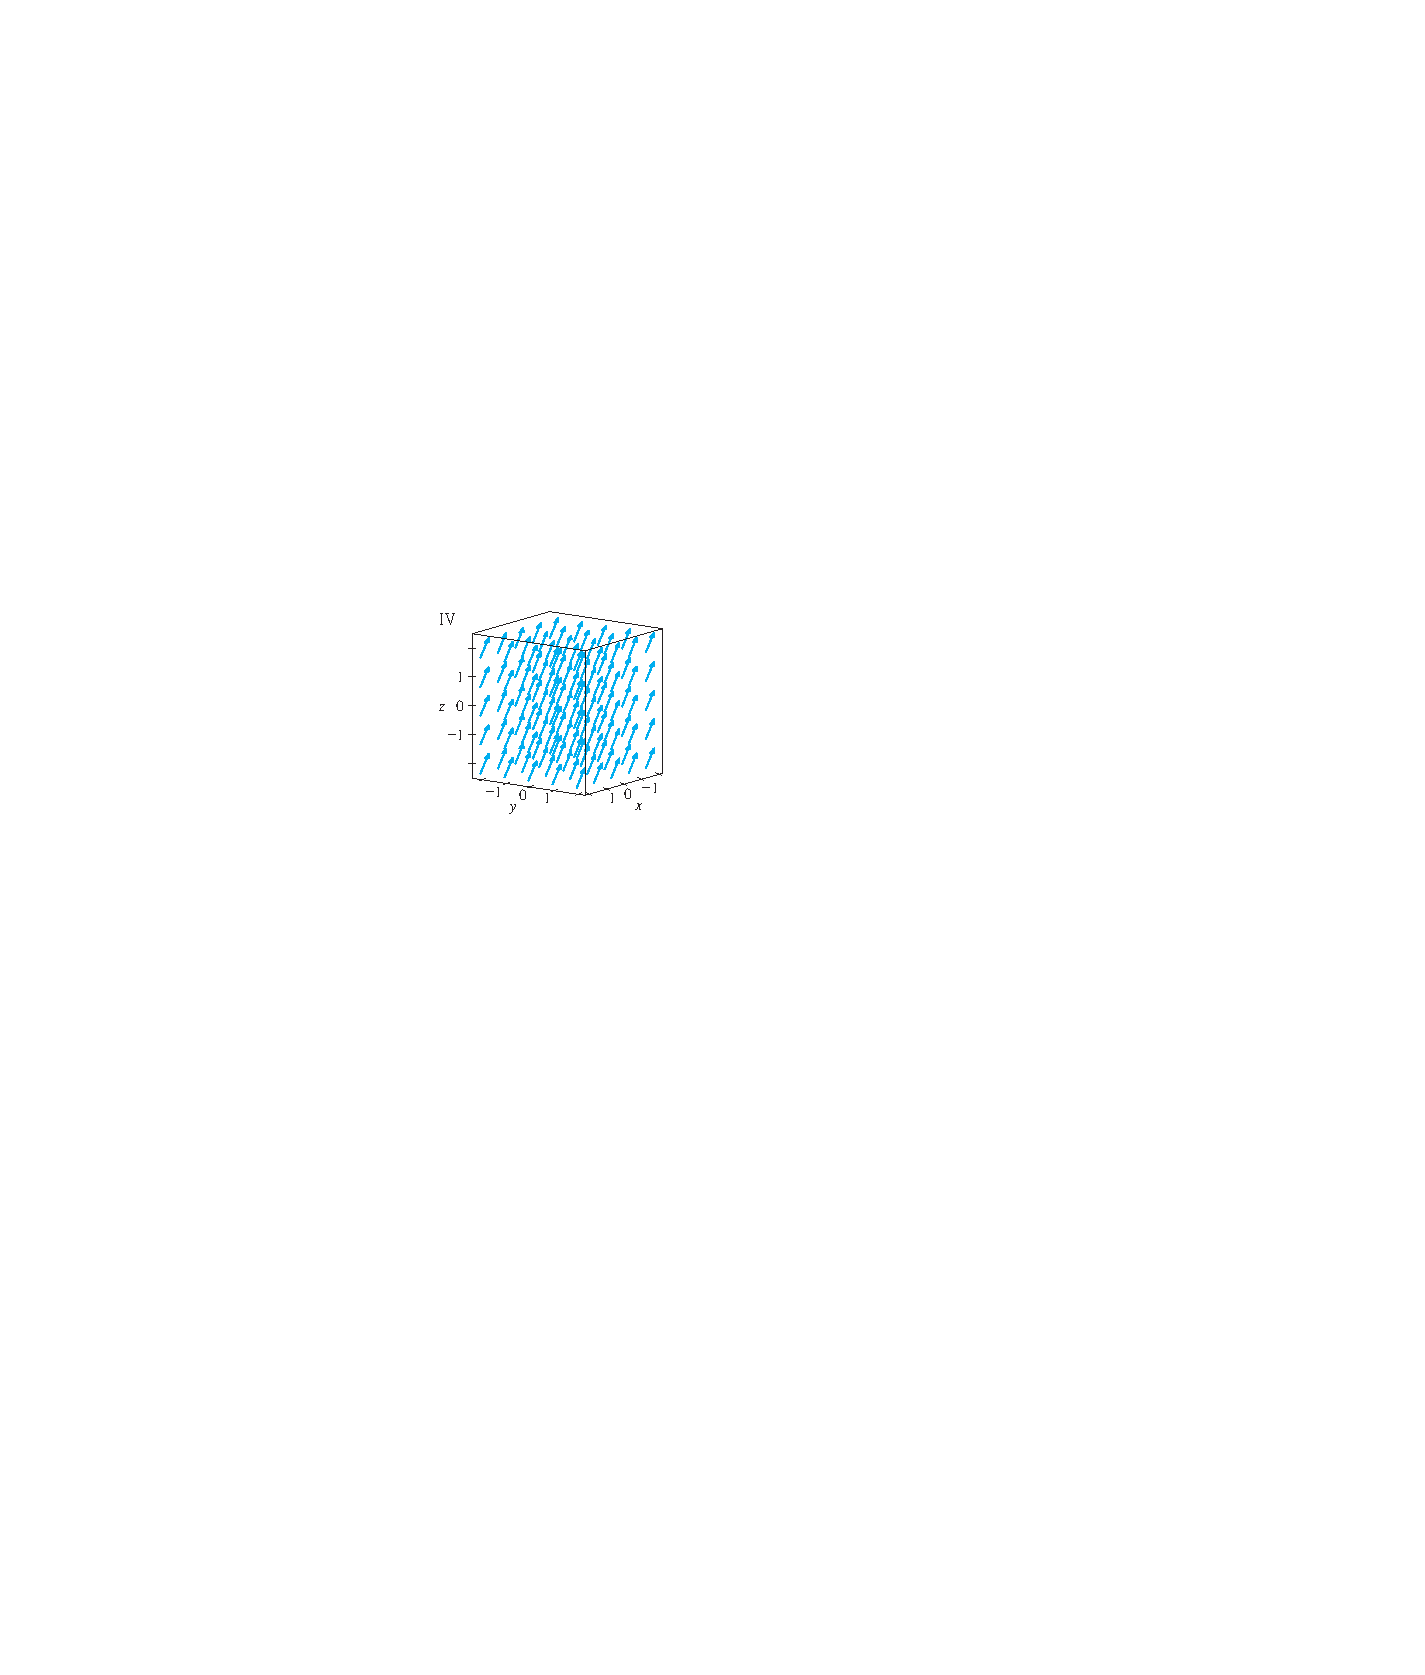
\includegraphics[scale=1.25]{IV.pdf}
\end{minipage}


\newpage
\prob Find formulas for the vectors fields below.

\bigskip
\begin{minipage}{0.5\textwidth}
\begin{itemize}
\item[(a)] \textcolor{white}{blank} \\

\includegraphics[scale=1.75]{pic1.pdf}\vspace{0.5in}
\item[(c)] \textcolor{white}{blank} \\

\includegraphics[scale=1.75]{pic3.pdf}\vspace{0.5in}
\item[(d)] \textcolor{white}{blank} \\

\includegraphics[scale=1.75]{pic4.pdf}
\end{itemize}
\end{minipage}
\begin{minipage}{0.5\textwidth}
\begin{itemize}
\item[(b)] \textcolor{white}{blank} \\

\includegraphics[scale=1.75]{pic2.pdf}\vspace{0.5in}
\item[(d)] \textcolor{white}{blank} \\

\includegraphics[scale=1.75]{pic5.pdf}\vspace{0.5in}
\item[(f)] \textcolor{white}{blank} \\

\includegraphics[scale=1.75]{pic6.pdf}
\end{itemize}
\end{minipage}

\newpage
\prob For each description of a vector field in parts (a)-(d), choose one or more of the vector fields (i)-(ix).

\bigskip
\begin{enumerate}
\item Pointing radially outward, increasing in length away from the origin.\vspace{0.5in}
\item Pointing in a circular direction around the origin, remaining the same length.\vspace{0.5in}
\item Pointing toward the origin, increasing in length farther from the origin.\vspace{0.5in}
\item Pointing clockwise around the origin.\vspace{0.5in}
\end{enumerate}

\begin{enumerate}[(i)]
\item $\displaystyle\frac{1}{\sqrt{x^2+y^2}}\begin{bmatrix}x \\ y \end{bmatrix}$\bigskip
\item $\displaystyle\frac{1}{\sqrt{x^2+y^2}}\begin{bmatrix}-y\\x \end{bmatrix}$\bigskip
\item $x\vec{i} + y \vec{j}$\bigskip
\item $-x\vec{i} - y \vec{j}$\bigskip
\item $\begin{bmatrix}-y \\ x \end{bmatrix}$\bigskip
\item $\begin{bmatrix}y \\ -x \end{bmatrix}$\bigskip
\item $\begin{bmatrix}y \\ x\end{bmatrix}$\bigskip
\item $\displaystyle\frac{x\vec{i} + y \vec{j}}{(x^2+y^2)^{3/2}}$\bigskip
\item $-\displaystyle\frac{x\vec{i} + y \vec{j}}{(x^2+y^2)^{3/2}}$
\end{enumerate}

\newpage
\prob Match the contour plots in (a)-(d) with the gradient fields in (i)-(iv).

\bigskip
\begin{minipage}{0.5\textwidth}
\begin{center}
\begin{enumerate}
\item\textcolor{white}{blank} \\

\includegraphics[scale=1.5]{pic11.pdf}\vspace{0.5in}
\item\textcolor{white}{blank} \\

\includegraphics[scale=1.5]{pic12.pdf}\vspace{0.5in}
\item\textcolor{white}{blank} \\

\includegraphics[scale=1.5]{pic13.pdf}\vspace{0.5in}
\item\textcolor{white}{blank} \\

\includegraphics[scale=1.5]{pic14.pdf}
\end{enumerate}
\end{center}
\end{minipage}\begin{minipage}{0.5\textwidth}
\begin{center}
\begin{enumerate}[(i)]
\item\textcolor{white}{blank} \\

\includegraphics[scale=1.5]{pic15.pdf}\vspace{0.5in}
\item\textcolor{white}{blank} \\

\includegraphics[scale=1.5]{pic16.pdf}\vspace{0.5in}
\item\textcolor{white}{blank} \\

\includegraphics[scale=1.5]{pic17.pdf}\vspace{0.5in}
\item\textcolor{white}{blank} \\

\includegraphics[scale=1.5]{pic18.pdf}
\end{enumerate}
\end{center}
\end{minipage}



\end{document}